
\documentclass[line,margin,hidelinks]{res}
\usepackage{verbatim}
\usepackage{hyperref}
\usepackage{fancyhdr}
\usepackage{graphicx}  % includegraphics
\usepackage{mathtools} % text
\hypersetup{colorlinks=true,
  urlcolor=blue,
  pdfauthor={Shawn F. Murphy},
  pdftitle={Resume of Shawn F. Murphy},
  pdfsubject={smurp}}
% TODO get pdfpagemode=UseOutlines to work by extending res.cls

%% \pagestyle{fancy}
%% \fancyhead{}
%%\fancyfoot{}
%% \fancyfoot[L] {\thepage}

\topmargin=-0.5in % start text higher on the page
\font\attand=cmr7

%
% Logos
% =====
\def\PS{{\tt P\small OST\tt S\small CRIPT}}
\def\ATT{{AT{\attand \&}T}}
\def\MF{{METAFONT}}
\def\Cplusplus{{\rm C\raise.5ex\hbox{\small ++}}}
\def\AmSTeX{{$\cal A\kern-.1667em\lower.5ex\hbox{$\cal M$}\kern-.125em
S$-\TeX}}

\begin{document}


\name{Shawn F. Murphy}
\address{
  \href{https://smurp.com}{smurp.com}\\
  Berlin \& Saltspring\\
   \href{https://www.linkedin.com/in/smurp}{linkedin.com/in/smurp}\\
   % \href{tel:+1-650-503-4034}{+1-650-503-4034}\\
   \href{tel:+49.160.462.8556}{+49.160.462.8556}\\
   {\tt \href{mailto:sfm@smurp.com}{sfm@smurp.com}}}

\resumewidth=7.2in
\sectionskip=.08in
\begin{resume}

\begin{format}
\dates{lm}\title{c}\employer{r}\\
% \dates{lm}\location{r}\\
% \body
\end{format}

%\begin{format}
%  \title{c}\\
%  \employer{l}\location{c}\\
%  \dates{r}\\
%  \body\\
%\end{format}

%%%%%%%%%%%%%%%%%%%%%%%%%%%%%%%%%%%%%%%%%%%%%%%%%%%%%%%%%%%%

\section{Profile:
  \newline   \newline
  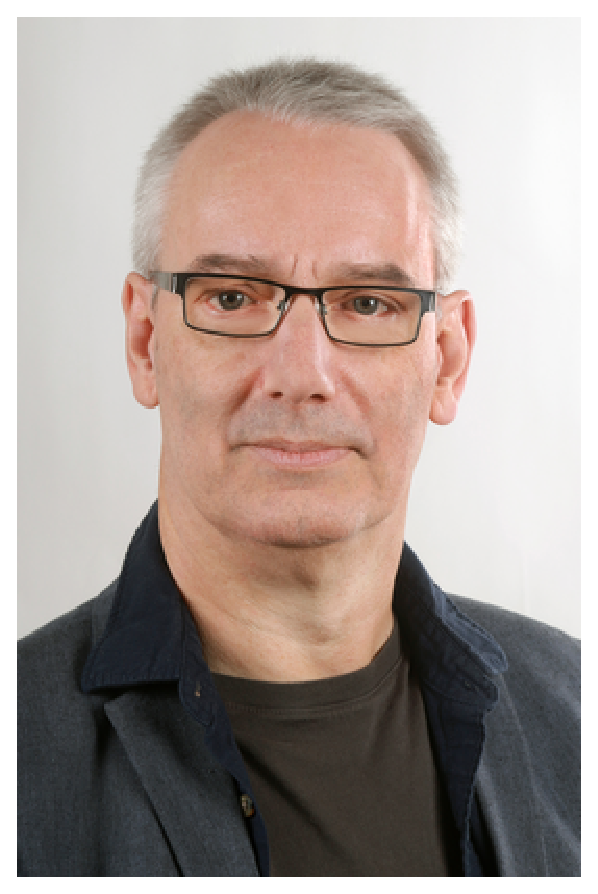
\includegraphics[width=1.1in]{mugshot.eps}}
\begin{par}

  Shawn Murphy is a visionary, innovative and goal-surpassing
  FOUNDER, CEO and CTO with 30+ years of successfully spearheading the
  execution of organization visions through bold and solutions-focused
  business strategies.
  \begin{itemize}
  \item \textbf{Software architect}, knowledge engineer,
    software \textbf{developer}, dev team leader,
    and trainer with vast experience designing and building large
    data-driven, scientific, academic, collaborative, e-commerce,
    visualization and publishing systems
  \item Highly proficient in diverse programming languages, knowledge
    representation technologies, frameworks, visualization tools, RDBMSes,
    ORMs, APIs, standards, methodologies and architectural styles
  \item Motivated by the observation that exponentiating technologies
    (A.I., computing, robotics, biosci) are dominating flatlining
    wisdom he has led research into solving the human-values
    alignment problem as a foundation for addressing AI alignment,
    democratic fragility, irreproducible science, fake news and other conundra
  \item A visionary leader striving to build out a global-scale
    knowledge management ecosystem wherein software, knowledge and
    presentation co-evolve under the pressure of human values and
    expertise -- to technologically host and ground our collective
    cognition, so we can meet the challenges of our time
  \end{itemize}

\begin{comment}
Examples of his work include:
  a vehicle fleet tracking system with RESTful API;
  multiple dynamic knowledge visualization systems;
  a custom database publishing system used by the largest real estate
    markets in Western Canada;
  real-estate systems powered by his own RETS implementation;
  a large bibliographic collaboration system seeded with Library of Congress data;
  a Laboratory Information Management System for disease diagnosis which
    captured, processed and reported on disparate scientific data streams;
  recruiting management systems;
  numerous B2B and B2C e-commerce technologies and systems
    (handling both digital and tangible goods);
  and many other projects involving sophisticated data-sets and processing.
\end{comment}

\end{par}


%%%%%%%%%%%%%%%%%%%%%%%%%%%%%%%%%%%%%%%%%%%%%%%%%%%%%%%%%%%%
\section{Professional Specialties:}
\begin{par}
Knowledge Representation \& Graphs,
Semantic Web,
Distributed Systems,
Collaborative Filtering,
Agile,
RDBMS,
EDI,
ORM,
Functional,
OOP,
Cognitive Computing,
Dynamic Graphics,
DevOps,
Pattern Languages,
Data-Context-Interaction,
Browser Extensions,
Identity Management,
NoSQL,
DevOps,
FOSS,
Computer Supported Collaborative Work
\end{par}

%%%%%%%%%%%%%%%%%%%%%%%%%%%%%%%%%%%%%%%%%%%%%%%%%%%%%%%%%%%%
\section{Standards:}
\begin{par}
TMDM,
OKBC,
RETS,
Digest Auth,
RBAC,
~ANSI~X12~EDI
\end{par}

%%%%%%%%%%%%%%%%%%%%%%%%%%%%%%%%%%%%%%%%%%%%%%%%%%%%%%%%%%%%
\section{Languages:}
\begin{par}
  Python, Javascript, Coffeescript, Typescript, Postscript, SQL, Rust, Bash,
  Java, C, AWK, ObjC, Scheme, Smalltalk, LISP, Nim
\end{par}

%%%%%%%%%%%%%%%%%%%%%%%%%%%%%%%%%%%%%%%%%%%%%%%%%%%%%%%%%%%%
\section{Formats:}
\begin{par}
  HTML5, CSS, SVG, XML, DocBook, SGML, Markdown, \LaTeX, N3, TriG
\end{par}

%%%%%%%%%%%%%%%%%%%%%%%%%%%%%%%%%%%%%%%%%%%%%%%%%%%%%%%%%%%%
\section{\footnotesize{Upper Ontologies:}}
\begin{par}
  RDF*, OWL, OKBC, TMAPI, CycL, WordNet, KQML, DAML
\end{par}


% \section{Languages, Formats, APIs and DTDs:}
% \begin{ncolumn}{5}
$\bullet$ Python
 &$\bullet$ Java
 &$\bullet$ HTML5
 &$\bullet$ Angular
 &$\bullet$ RDF*\\

$\bullet$ Javascript
 &$\bullet$ C
 &$\bullet$ CSS
 &$\bullet$ React
 &$\bullet$ OWL\\

$\bullet$ Typescript
 &$\bullet$ AWK
 &$\bullet$ SVG
 &$\bullet$ Selenium
 &$\bullet$ SPARQL\\

$\bullet$ Coffeescript
 &$\bullet$ ObjC
 &$\bullet$ XML
 &$\bullet$ DocBook
 &$\bullet$ N3\\

$\bullet$ Postscript
 &$\bullet$ Scheme
 &$\bullet$ jQuery/UI
 &$\bullet$ SGML
 &$\bullet$ TriG\\

$\bullet$ SQL
 &$\bullet$ Smalltalk
 &$\bullet$ D3
 &$\bullet$ \LaTeX
 &$\bullet$ OKBC\\

$\bullet$ Bash
 &$\bullet$ LISP
 &$\bullet$ $<${\tt canvas}$>$
 &$\bullet$ Markdown
 &$\bullet$ TMAPI\\

$\bullet$ Rust
 &$\bullet$ Nim
 &$\bullet$ ${\tt 2d/webgl}$
 &$\bullet$ Make
 &$\bullet$ CTM\\

\end{ncolumn}




%%%%%%%%%%%%%%%%%%%%%%%%%%%%%%%%%%%%%%%%%%%%%%%%%%%%%%%%%%%%
\section{Systems:}
\begin{par}
Linux MacOS iOS Android Squeak Minix AS/400 OS/2 NeXTstep Windows AppleII
\end{par}

%%%%%%%%%%%%%%%%%%%%%%%%%%%%%%%%%%%%%%%%%%%%%%%%%%%%%%%%%%%%
\section{Industries:}
\begin{par}
Artificial Intelligence,
Molecular Nanotechnology,
Bioinformatics,
Bibliographic Systems,
Digital Humanities,
B2B \& B2C E-Commerce,
Database Publishing,
Real Estate,
Recruiting Systems,
Fleet Automation \& Tracking,
Supply Chain Automation,
Laboratory Information Management,
Learning Management
\end{par}

%%%%%%%%%%%%%%%%%%%%%%%%%%%%%%%%%%%%%%%%%%%%%%%%%%%%%%%%%%%%

\section{Experience}

\title{ Founder \& CEO }
\location{ Edmonton, Saltspring, Berlin }
\employer{ \href{https://nooron.com}{Nooron Collaboratory Inc/UG} }
\dates{2015 to present}


\title{ Fullstack Software Engineer }
\location{ Orange County, California }
\employer{ \href{https://web.archive.org/web/20140214033414/https://www.connectifier.com/about}{Connectifier} }
\dates{2013 to 2014}
\begin{position}
Used Java, Scala, AngularJS, the Play Framework, MongoDB, Elastic
Search and Selenium as part of a startup team to build a category
leading recruiting platform.  Connectifier used big data and machine
learning techniques to crawl the web and social networks for CV and
contact information to empower recruiters specialized in hiring
software engineering talent.  Shawn was their sixth engineer following
the four initial Google software engineers.  Shawn left to found Nooron
Collaboratory.  Connectifier was later acquired by LinkedIn.
\end{position}


\title{ Architect \& Programmer }
\employer{ \href{https://www.artsrn.ualberta.ca/orlando/}{The Orlando Project} }
\location {Universities of Alberta, Guelph \& McGill}
\dates{2013 to 2014}
\begin{position}
Coding and architecting an animated highly interactive semantic
visualization research platform using D3, Canvas, RDF and NodeJS for a
university consortium working in the digial humanities.  It features
multi-modal interactivity ( using direct manipulation; bulk
specification and a novel semantic graph layout specification language
) to support visual exploration of a large text corpus.
\end{position}


\title{ Founder, CTO, Architect }
\location{ Saltspring Island \& Edmonton}
\employer{ \href{https://web.archive.org/web/20141009141222/http://semandra.com:80/}{Semandra, Inc.} }
\dates{2011 to 2014}
\begin{position}
Semandra provided full-service front-to-backend
website development specializing in graphics-intensive designs with
multimedia integration, database-driven backends with complex
programming requirements, and content-rich user-maintainable CMS
sites.

\begin{itemize}
  \item Ponderate --- an agile, collective knowledge curation and evaluation tool
  \item TOBFleet --- a RESTful web service which simplifies vehicle fleet integrations
  \item Theamatic --- a web application for repertory theatre and film
    festival management.
  \item CReturns --- a graphical scheduling system, e-commerce
    solution and SalesForce integration for this home energy auditing and
    retrofitting service
\end{itemize}

\end{position}



\title{ Principal }
\location{Edmonton, AB}
\employer{ \href{http://smurp.com}{smurp.com} }
\dates{2002 to 2011}

\begin{position}
Smurp.com provided contract programming and consulting services with a focus
on database-backed web sites and complex data processing operations.

\begin{itemize}
%  \item Nooron --- an experimental knowledge publishing and collaboration
%    environment featuring knowledge-based web-apps such as:
%    project management, pattern languages, blogging and FAQs.
%    It published knowledge within and about itself in various textual
%    and graphical forms:
%    DocBook, Rich Text, SVG, GIF, JPG, PDF and Postscript;
%    UML diagrams; state-transition diagrams; network graphs;
%    inheritance trees and PERT charts.

  \item PyOKBC --- A Python implementation of the
     \emph{Open KnowledgeBase Connectivity}
  system of knowledge representation and abstraction.
  It was designed to provide a single consistent interface to diverse structured
  information sources, to include ontologies, relational databases,
  xml documents, and topic maps. % PyOKBC was Free Software under the LGPL.

  \item PyRETS --- An implementation of the \emph{Real Estate Transaction System}
  for keeping the Vancouver Real Estate Board synchronized with MLS.ca

  \item CatPub --- A database publishing technology consisting of a
  Postscript templating system over a relational database back-end.
  Suitable for automatically preparing complex, highly customized,
  Postscript and PDF publications such as directories and catalogs,
  it is closed source software created under contract for a firm
  providing publishing services to the real estate industry.
  It is producing on the order of 10 thousand unique catalog pages
  every day containing constantly changing data for the largest
  real estate boards in Western Canada.

  \item TKQ2.0 --- A Django e-store system vending e-books for hundreds
  of educational publishers, through a dozen store-fronts, with sophisticated
  features such as promotions, steganographic watermarking in PDF, bundling,
  coupons and more.

  \item TKQW --- A Medusa-based ``digital drop-shipping`` system
  enabling digital goods sale and delivery by untrusted 3rd parties.

  \item ModelViz --- Added dynamic SVG-based touring facilities to this Django
  model entity-relationship visualizer.

  \item Alberta Lodging Association --- A Django-based lodgings database
  backing a web site, a printed directory and an associated advertising
  sales and layout system.

\end{itemize}

\end{position}




\begin{position}
  \title{ Founder, Chair, VP R\&D }
  \location{Edmonton, AB}
  \employer{ \href{https://web.archive.org/web/20000824074057/http://emergence.com/}{Emergence by Design} }
  \dates{1995 to 2003}
  
  Shawn founded Emergence by Design along with four colleagues to pursue
  the development of \emph{The Idea Engine}.  To fund the ongoing development of
  TIE, EbD became a dot-com factory, providing consulting,
  development, hosting and ecommerce services to new dot-com ventures.
  Shawn was VP of R\&D, lead developer and chief architect of this 15-person
  organization, until selling his interest in 2003.

\begin{itemize}

\item TheIdeaEngine --- architect and lead developer of this R\&D project
  developing a distributed knowledge representation system using
  Java (and JDBC), Perl (and DBI), Scheme, and various SQL backends.
  The effort included the
  implementation of the OKBC (Open Knowledge Base Connectivity)
  specification in Java and Perl,
  the authoring of a multithreaded knowledge server
  and the creation of many perl CGIs, Java Applets and Applications.

\item \href{https://web.archive.org/web/20140517102110/http://getcited.org/}{GetCited.org}
  --- chief architect and lead developer on this massive, highly abstracted
      academic bibliographic portal system featuring:
  \begin{itemize}
    \item reference and citation cross-references
    \item per-publication discusion forums
    \item curriculum vitae management
    \item links with Amazon and other vendors for associate
    referral income
    \item seeded with MARC Book and Serials databases from Library of Congress
    \item rich array of publication types (proceedings, books, articles,
       manuscripts, bibliographies, etc)
    \item tracking of individual/institutional affiliations
    \item sophisticated statistics on publishing influence of
       nations, institutions and individuals based on citation counts
  \end{itemize}

\item \href{https://web.archive.org/web/20130302232056/http://www.dedicatedteacher.com/}{DedicatedTeacher.com}
   --- architect and lead developer
  for this large, highly abstracted ecommerce engine featuring:
    \begin{itemize}
      \item sells both 'digital-goods' (eg. MP3s and PDFs of books)
      and 'tangible goods' (printed books, CDs, educational kits)
      \item complex shipping options
      \item multiple suppliers per store
      \item sophisticated coupon, bundle, sale and promotion features
      \item serves store fronts for various companies
      (e.g. Scholastic)
      \item supports multiple currencies, multiple credit-card
      transaction backends simultaneously and selectively
      (depending on currency, card-type, availability, etc.)
    \end{itemize}

\item \href{https://web.archive.org/web/19991205174419/http://www.lawopinion.com/}{Law Opinion}
   --- architect and developer of the worlds first E-Commerce facility for
       the provision of paid legal opinions.
       It included numerous encryption safeguards
       to ensure complete client confidentiality; a
       system for letting people pick the nearest
       lawyer with experience in the chosen area of
       the law;  and a sophisticated, dynamic,
       system for performing branching automated interviews.
\item \href{http://findamentor.com/}{FindAMentor.com}
   --- architect and lead developer of this system
       for helping people find and interact with mentors in
       various areas of their lives; complete with anonymization and
        multiple personal profiles in different areas of interest
\item EmailDirector
   --- architect and developer of this web-based school management
       system with parallel web and email interfaces
       and sophisticated email transaction system for,
       at that time, Canada's largest e-school
       with 2500 grade-school students
\item EStore
   --- architect and developer of this web interface for creating E-Commerce
       websites using NGage Electronic Commerce technology
\item recruiter matchmaking system
   --- salvaged, re-architected and built out a head-hunting firm's
       matchmaking system for staffing high-tech jobs based on skill, locality
       and position type
\item ClickTrace --- architect and developer of this web log mining facility
\item Domainatrix --- architect and developer of this
                      toolset for bulk management of domain registrations,
                      DNS configurations and network interface
                      configuration
\item Edmonton Chamber of Commerce Annual Directory ---
         architect of this database-driven directory
         including ads and equivalents of white pages and yellow pages
\item magazine publishing system ---
  architect of this complete publishing solution
  with extensive features for advertising sales management and ad layout
  automation

\end{itemize}

\end{position}


\title{Systems Analyst I, II \& III}
\location{ Edmonton, AB}
\dates{1989 to 1995}
\employer{Gov't of Alberta}
\begin{position}
  Shawn was responsible for analysis, design, programming,
  training and support of LABBASE: a multi-disciplinary LIMS
  (Laboratory Information Management System) coded in Paradox and
  WordBasic.  It co-operated with a legacy AS/400 appliction written
  in RPG/400 and CL, which he also maintained.  During this project he
  managed three other programmers, the AS/400 administrator and a tech
  support person.
\end{position}


\title{ Principal }
\location{ Edmonton, AB}
\dates{1990 to 1995}
\employer{Sapient Systems}
\begin{position}
Sapient Systems specialized in the creation of desktop database apps.
\begin{itemize}
\item Wrote {\it FastEDI} in PAL (the Paradox Application Language)  to
	provide a subset of the
	ANSI X.12 (V3.020) Electronic Data Interchange system for an
	oilfield supply company interested in easing the ordering process for
	the many regional offices of their large clients in the oil patch.
	{\it FastEDI v1.0} implemented
	the transaction sets for Price/Sales Catalog (832) and
	Purchase Order (850) thus enabling the electronic distribution
	of the latest pricelist and placement of orders.
\item Created a {\it Disability Inventory \& Assessment System }
	for an Educational Consultant to use as a proof of concept of
	her doctoral work for possible productization.
\item Created a {\it Property Management System} for a Realty Firm to
	track the features, locations, prices and owners of
	available commercial real estate to facilitate showing to clients
\item Attended ``NeXT Developer Camp`` and wrote \emph{Elements.app}
\end{itemize}
\end{position}


\title{ Founder \& Director }
\location{ Edmonton, AB}
\employer{TechnoWatch Society}
\dates{1990 to 1992}
\begin{position}
  Founded and managed this non-profit think tank focused on the strategic impacts of
  emerging technologies such as nanotech, biotech, AI and robotics.
  Put on presentations, guided staff, and conducted a scientific literature review.
\end{position}





%%%%%%%%%%%%%%%%%%%%%%%%%%%%%%%%%%%%%%%%%%%%%%%%%%%%%%%%%%%%
% \section{Education:}
% \begin{format}
% \title{l}\\
% \dates{l}\location{r}\\
% \body\\
% \end{format}

% \title{ Educational Background }
% \begin{itemize}
% \item Lester B Pearson, United World College of the Pacific, 1980-1982
% \item University of Alberta, 1982/83, 1985/86
% \item Saskatchewan Inst. of Applied Science \& Technology, 1988
% \item NeXT Inc. ``NeXT Developer Camp``, 1991
% \end{itemize}

% \title{ Networking and Professional Development }
% \employer{}
% \location{ Silicon Valley }
% \dates{1990 to present}
% \begin{position}
% At least twice a year over the last twenty years, Shawn has participated
% in diverse cutting-edge professional and scientific gatherings -- 
% and conducted personal interviews with thought leaders -- in nanotechnology, 
% artificial intelligence, science and public policy, biotechnology, 
% quantified self, semantic web, open source software and singularity studies.
% \end{position}


% \title{ NeXT Inc. }
% \employer{}
% \location{ Redwood City, CA}
% \dates{Spring 1991}
% \begin{position}
% 'Developer Camp': training in Object Oriented Analysis and Development in 
% Objective-C on the NeXT Unix workstation.
% \end{position}

% \title{ Sask. Inst. of Applied Science \& Technology}
% \location{ Prince Albert, SK}
% \dates{Fall 1988}
% \begin{position}
% Micro-Electronics Technician certificate program.  This one year
% Competency-Based Education course was completed in 3 months.  This course
% was taken to counterbalance a growing software-centricity.  Design, 
% construction and degbugging of digital electronic systems.
% \end{position}

% \title{ University of Alberta}
% \location{ Edmonton, AB}
% \dates{1982/83, 1985/86}
% \begin{position}
% Courses in General Science including Honors Math, Honors Physics,
% Computing Science and Philosophy.
% \end{position}

% \title{ United World College of the Pacific}
% \location{ Victoria, BC}
% \dates{1980-1982}
% \begin{position}
% Received the International Baccaluareate: a first year university 
% equivalent liberal arts degree with Higher Levels in Physics, 
% Math and English; Subsidiary Levels in Economics, Art and Philosophy 
% in French.  Extracurricular activities included: 
% programming Apple II and Hewlet Packard microcomputers; 
% playing lead male role and being technical director in a large 
% semi-professional theatrical production of 
% Bertolt Brecht's {\it Mother Courage}.
% \end{position}


% \title{ Samual Hearne Secondary School}
% \location{ Inuvik, NT}
% \dates{1976-1980}
% \begin{position}
% Went to college instead of grade 12;
% Student Council member; skipped grade 9; programmed TRS-80 microcomputer 
% and TI-59; represented (at age 14) 
% Northwest Territories at the 1978 Canadian National (highschool) Debate Championship.
% \end{position}


%%%%%%%%%%%%%%%%%%%%%%%%%%%%%%%%%%%%%%%%%%%%%%%%%%%%%%%%%%%%
 \section{Interests:}
 \begin{ncolumn}{4}
 $\bullet$ A-Life      &$\bullet$ Agorics   &$\bullet$ Autopoesis    &$\bullet$ Design Patterns  \\
 $\bullet$ Emergence   &$\bullet$ Evolution &$\bullet$ Planetworking &$\bullet$ Quantified Self \\
 $\bullet$ Game Theory &$\bullet$ GroupWare &$\bullet$ ISO-9000      &$\bullet$ Markets \\
 $\bullet$ Nanotech    &$\bullet$ Noosphere &$\bullet$ Singularity   &$\bullet$ Wearables \\
 \end{ncolumn}

\end{resume}
\end{document}

